% =====================================================================
%  Relazione di progetto -- Programmazione su Architetture Parallele
%  Compilare con:  pdflatex relazione.tex   (due volte, per i riferimenti)
% =====================================================================
\documentclass[11pt,a4paper]{article}

\usepackage[utf8]{inputenc}
\usepackage[T1]{fontenc}
\usepackage[italian]{babel}
\usepackage{lmodern}
\usepackage[margin=2.6cm]{geometry}
\usepackage{amsmath}
\usepackage{amssymb}
\usepackage{booktabs}
\usepackage{graphicx}
\usepackage{listings}
\usepackage{xcolor}
\usepackage{algorithm}
\usepackage{algpseudocode}
\usepackage[hidelinks]{hyperref}

% margine di elasticita': gli identificatori in \texttt{} non sono sillababili
\setlength{\emergencystretch}{3em}

% ---- marcatore per le parti non ancora scrivibili -------------------
\newcommand{\daFare}[1]{%
  \par\vspace{2pt}%
  \noindent\fcolorbox{red!60!black}{red!6}{%
    \begin{minipage}{0.97\linewidth}
    \textbf{\textcolor{red!60!black}{[DA COMPLETARE]}}\quad #1
    \end{minipage}}%
  \par\vspace{4pt}%
}

% ---- stile per i listati di codice ----------------------------------
\definecolor{cmtgray}{gray}{0.45}
\lstset{
  basicstyle=\ttfamily\footnotesize,
  commentstyle=\color{cmtgray}\itshape,
  keywordstyle=\bfseries,
  numbers=left, numberstyle=\tiny\color{gray}, numbersep=7pt,
  frame=leftline, framesep=6pt, xleftmargin=14pt,
  breaklines=true, showstringspaces=false, captionpos=b
}

\title{\textbf{PageRank su Architetture Ibride}\\[2mm]
       \large Parallelizzazione con OpenMP e CUDA}
\author{Emanuele Cecchia}
\date{Corso di Programmazione su Architetture Parallele\\
      A.A.\ 2025--26 --- Prof.\ Andrea Formisano\\[2mm]\today}

\begin{document}
\maketitle

% =====================================================================
\section*{Abstract}
% =====================================================================
Il progetto implementa e analizza l'algoritmo PageRank su architetture
parallele, confrontando tre versioni: una sequenziale, che fa da
riferimento per ogni misura di speed-up, una puramente multicore basata su
OpenMP e una ibrida che distribuisce il carico fra CPU e GPU tramite CUDA.
Sequenziale e OpenMP condividono lo stesso file sorgente e differiscono
solo per le opzioni di compilazione, così che il riferimento non possa
divergere dal codice parallelo né essere falsato dai costi di gestione dei
thread. Il grafo è memorizzato in formato CSR trasposto, scelta che rende il
nucleo di calcolo privo di scritture concorrenti e quindi parallelizzabile
senza sincronizzazione. La correttezza è verificata contro tre
implementazioni indipendenti. Le misure sulla versione OpenMP mostrano uno
speed-up di $2{,}4$--$2{,}9\times$ su 4 core fisici e, soprattutto, una
saturazione oltre i 4 thread che identifica il calcolo come
\emph{memory-bound}: è questo il dato che motiva quantitativamente il
passaggio alla GPU.

\daFare{Aggiornare l'abstract con i risultati CUDA una volta completata la
fase ibrida.}

\tableofcontents
\newpage

% =====================================================================
\section{Descrizione del problema affrontato}
% =====================================================================

\subsection{Il problema}
PageRank assegna a ogni nodo di un grafo orientato un punteggio di
importanza, definito ricorsivamente: un nodo è importante se nodi
importanti puntano ad esso. Nato per ordinare le pagine web in base alla
struttura dei collegamenti ipertestuali~\cite{page1999}, viene oggi
applicato anche a reti sociali, reti di citazioni e reti biologiche.

La definizione è ricorsiva e si risolve iterativamente: si parte da una
distribuzione uniforme e la si raffina finché non cambia più --- in
pratica, finché la variazione non scende sotto una soglia prefissata,
oppure fino a un numero massimo di iterazioni. Equivale al
modello del \emph{navigatore casuale}, che segue collegamenti scelti a caso:
il PageRank è la frazione di tempo che costui trascorre su ciascuna pagina.
Ne discendono due proprietà della formula --- il totale vale 1, perché il
navigatore è sempre da qualche parte, e un collegamento pesa tanto meno
quanti più ne partono dalla stessa pagina.

Formalmente, dato un grafo orientato $G=(V,E)$ con $N=|V|$,
\begin{equation}
\mathrm{PR}_{t+1}(v) \;=\; \frac{1-d}{N}
\;+\; d\left( \sum_{u \,:\, u \to v} \frac{\mathrm{PR}_t(u)}{\mathrm{outdeg}(u)}
\;+\; \frac{\mathrm{DM}_t}{N} \right)
\label{eq:pagerank}
\end{equation}
dove i simboli hanno il seguente significato:
\begin{center}
\begin{tabular}{@{}ll@{}}
\toprule
$\mathrm{PR}_t(v)$ & \emph{PageRank}: punteggio del nodo $v$ alla $t$-esima iterazione \\
$\mathrm{outdeg}(u)$ & numero di archi uscenti da $u$ \\
$d$ & \emph{damping factor}, convenzionalmente $0{,}85$ \\
$\mathrm{DM}_t$ & \emph{dangling mass}: punteggio complessivo dei nodi senza archi uscenti \\
 & $\mathrm{DM}_t=\sum_{u\,:\,\mathrm{outdeg}(u)=0}\mathrm{PR}_t(u)$ \\
$N$ & numero di nodi \\
\bottomrule
\end{tabular}
\end{center}

\subsection{Il termine dangling}
Il termine $\mathrm{DM}_t/N$ non è un dettaglio implementativo ma una necessità
matematica. Un nodo senza archi uscenti non ha modo di ridistribuire il
proprio rank: ignorandolo, ad ogni iterazione una frazione della massa
totale sparirebbe e il vettore cesserebbe di essere una distribuzione di
probabilità. Nei dataset utilizzati questo non è un caso limite: il
$15{,}6\%$ dei nodi di \texttt{web-Google} e l'$11{,}1\%$ di
\texttt{soc-LiveJournal1} sono dangling (Tabella~\ref{tab:dataset}).

La conseguenza pratica è che $\sum_v \mathrm{PR}(v) = 1$ costituisce un test di
correttezza immediato e molto sensibile: il programma lo stampa ad ogni
esecuzione.

\subsection{Forma matriciale}
\label{sec:matriciale}

La stessa iterazione si scrive in forma vettoriale. Sia $\mathbf{MT} \in \mathbb{R}^{N \times N}$ la \emph{matrice di
transizione} definita da
\begin{equation}
\mathrm{MT}_{vu} =
\begin{cases}
1/\mathrm{outdeg}(u) & \text{se esiste l'arco } u \to v,\\[2pt]
0 & \text{altrimenti,}
\end{cases}
\end{equation}
e sia $\mathbf{1}$ il vettore di tutti uni. Detto $\mathbf{PR}_t$ il
vettore dei punteggi, l'iterazione~\eqref{eq:pagerank} diventa
\begin{equation}
\mathbf{PR}_{t+1} \;=\; \frac{1-d}{N}\,\mathbf{1}
\;+\; d\left( \mathbf{MT}\,\mathbf{PR}_t + \frac{\mathrm{DM}_t}{N}\,\mathbf{1} \right),
\qquad \mathrm{DM}_t = \mathbf{w}^{\!\top} \mathbf{PR}_t
\label{eq:matriciale}
\end{equation}
dove $\mathbf{w}$ è il vettore indicatore dei nodi dangling ($w_u=1$ se
$\mathrm{outdeg}(u)=0$, altrimenti $0$).

Ogni colonna di $\mathbf{MT}$ somma a 1, tranne quelle dei nodi dangling che
sono nulle: è questa mancanza a richiedere il termine correttivo. La
formulazione classica lo assorbe in un'unica \emph{matrice di Google}
\begin{equation}
\mathbf{G} \;=\; d\left(\mathbf{MT} + \tfrac{1}{N}\mathbf{1}\mathbf{w}^{\!\top}\right)
\;+\; \tfrac{1-d}{N}\,\mathbf{1}\mathbf{1}^{\!\top},
\qquad \mathbf{PR} = \mathbf{G}\,\mathbf{PR}.
\end{equation}
$\mathbf{G}$ è stocastica per colonne e positiva, quindi per Perron--Frobenius
ha autovalore dominante 1 con autovettore unico: il PageRank \emph{è}
quell'autovettore, e l'iterazione è il \emph{metodo delle potenze} applicato
a $\mathbf{G}$.

\paragraph{Perché non si costruisce $\mathbf{G}$.}
$\mathbf{G}$ è elegante ma inutilizzabile: i termini
$\mathbf{1}\mathbf{w}^{\!\top}$ e $\mathbf{1}\mathbf{1}^{\!\top}$ sono densi,
quindi avrebbe $N^2$ non nulli --- $5{,}6$~TB per \texttt{web-Google}. Si usa
perciò la forma~\eqref{eq:matriciale}, dove l'unica matrice è $\mathbf{MT}$,
sparsa e memorizzata in CSR (Sezione~\ref{sec:csr}), mentre i contributi
densi si riducono a due scalari. Il prodotto $\mathbf{MT}\,\mathbf{PR}_t$ è
una moltiplicazione matrice-sparsa per vettore (SpMV): è questa l'operazione
che il progetto parallelizza.

\subsection{Algoritmo sequenziale}
\begin{algorithm}[H]
\caption{PageRank per iterazione di potenza (formulazione \emph{pull})}
\label{alg:seq}
\begin{algorithmic}[1]
\State $\mathrm{PR}(v) \gets 1/N$ \textbf{per ogni} $v \in V$
\Repeat
  \State $\mathrm{DM} \gets 0$
  \ForAll{$u \in V$}
    \If{$\mathrm{outdeg}(u) = 0$}
      \State $c(u) \gets 0$; \quad $\mathrm{DM} \gets \mathrm{DM} + \mathrm{PR}(u)$
    \Else
      \State $c(u) \gets \mathrm{PR}(u)/\mathrm{outdeg}(u)$
    \EndIf
  \EndFor
  \State $\mathit{base} \gets (1-d)/N + d\cdot \mathrm{DM}/N$
  \ForAll{$v \in V$}
    \State $\mathrm{PR}'(v) \gets \mathit{base} + d \sum_{u \to v} c(u)$
  \EndFor
  \State $\varepsilon \gets \sum_v |\mathrm{PR}'(v)-\mathrm{PR}(v)|$
  \State scambia $\mathrm{PR}$ e $\mathrm{PR}'$
\Until{$\varepsilon < \mathit{tolleranza}$}
\end{algorithmic}
\end{algorithm}

Il calcolo di $c(u)$ è separato dal ciclo di accumulo per una ragione di
costo: eseguito così richiede $N$ divisioni per iterazione anziché $M=|E|$,
e nei grafi considerati $M \gg N$ (su \texttt{soc-LiveJournal1}, 69 milioni
contro 4,8 milioni). La divisione è fra le operazioni aritmetiche più lente,
quindi il risparmio è reale.

\subsection{Necessità della parallelizzazione}
La difficoltà del problema è interamente di scala. Il grafo non può essere
rappresentato con una matrice densa $N \times N$: per \texttt{web-Google}
servirebbero $875\,713^2 \times 8$ byte $\approx 5{,}6$~TB, di cui oltre il
$99{,}99\%$ occupati da zeri, dato che il grado medio è circa 6. È quindi
necessaria una rappresentazione sparsa, e il calcolo va distribuito su più
unità di elaborazione per ottenere tempi accettabili al crescere
dell'istanza.

% =====================================================================
\section{Metodologia adottata per la soluzione}
% =====================================================================

\subsection{Rappresentazione dei dati: CSR trasposto}
\label{sec:csr}

Il grafo è memorizzato in formato \textbf{CSR} (Compressed Sparse Row) con
tre array:
\begin{itemize}
  \item \texttt{row\_ptr[N+1]}: offset di inizio di ogni riga;
  \item \texttt{col\_idx[M]}: i vicini, concatenati riga per riga;
  \item \texttt{out\_deg[N]}: grado uscente di ogni nodo.
\end{itemize}
I vicini del nodo $v$ occupano \texttt{col\_idx[row\_ptr[v] \dots
row\_ptr[v+1]-1]}. Un nodo privo di vicini ha
\texttt{row\_ptr[v] == row\_ptr[v+1]}: il ciclo semplicemente non viene
eseguito, senza bisogno di alcun caso speciale.

\paragraph{Perché il trasposto.}
La scelta progettuale più importante del progetto è \emph{quale} indice
diventa la riga. L'equazione~\eqref{eq:pagerank} richiede, per calcolare
$\mathrm{PR}_{t+1}(v)$, l'insieme dei nodi che puntano a $v$. Esistono due modi di
organizzare il calcolo:

\begin{description}
  \item[Push] si scorre l'insieme degli archi $u \to v$ e si somma il
    contributo di $u$ dentro $\mathrm{PR}'(v)$. Più archi convergono sullo stesso
    $v$, quindi più thread scrivono sulla stessa cella: si genera una
    \emph{race condition} che richiede operazioni atomiche o lock.
  \item[Pull] si scorre l'insieme dei nodi $v$, si leggono i suoi
    predecessori e si scrive $\mathrm{PR}'(v)$ una sola volta. Ogni nodo è di
    competenza di un solo thread: \textbf{non esiste alcuna scrittura
    concorrente}.
\end{description}

È stata adottata la formulazione \emph{pull}, che richiede di memorizzare,
per ogni nodo, la lista dei predecessori --- cioè il grafo con tutti gli
archi invertiti, il \emph{trasposto}. L'inversione non richiede un passo
dedicato: costruendo il CSR si sceglie semplicemente il nodo di
destinazione, anziché quello di origine, come indice di riga.

La motivazione è tanto più forte sulla GPU: le atomiche necessarie alla
variante \emph{push} serializzerebbero il kernel proprio sui nodi \emph{hub},
e \texttt{web-BerkStan} contiene un nodo con $84\,208$ archi entranti.

\paragraph{Costo evitato.}
Con la rappresentazione sparsa \texttt{web-Google} occupa 29,5~MB anziché i
5,6~TB della matrice densa.

\subsection{Formato binario e pre-elaborazione}
La conversione dal formato testuale SNAP al CSR avviene \emph{una volta
sola}, offline, tramite \texttt{tools/snap\_to\_csr.py}. Le motivazioni sono
due:
\begin{enumerate}
  \item l'analisi del testo è lenta e irregolare; eseguirla dentro il
    programma misurato significherebbe misurare il parser anziché
    l'algoritmo;
  \item il codice C non ha così bisogno di alcun parser testuale, il che
    elimina un'intera classe di errori dalla parte valutata.
\end{enumerate}

Gli identificatori SNAP sono sparsi (\texttt{web-Google} ha $875\,713$ nodi
con id fino a $916\,428$) e vengono rimappati su un intervallo contiguo
$[0,N)$; la corrispondenza inversa è salvata in un file \texttt{.ids}
separato, letto solo per riportare i risultati negli identificatori
originali.

Il formato binario prodotto è il seguente:
\begin{center}
\begin{tabular}{@{}lll@{}}
\toprule
\textbf{Campo} & \textbf{Tipo} & \textbf{Dimensione} \\
\midrule
magic \texttt{"PRCSR001"} & \texttt{char[8]}   & 8 byte \\
\texttt{n\_nodes}         & \texttt{uint64}    & 8 byte \\
\texttt{n\_edges}         & \texttt{uint64}    & 8 byte \\
\texttt{row\_ptr}         & \texttt{uint64[]}  & $8(N{+}1)$ byte \\
\texttt{col\_idx}         & \texttt{uint32[]}  & $4M$ byte \\
\texttt{out\_deg}         & \texttt{uint32[]}  & $4N$ byte \\
\bottomrule
\end{tabular}
\end{center}

\texttt{col\_idx} usa 32 bit anziché 64 perché gli elementi sono $M$: su
\texttt{soc-LiveJournal1} la scelta dimezza l'occupazione da 552~MB a
276~MB, ed è sicura perché un indice di nodo è sempre minore di
$N < 2^{32}$. Il caricamento lato C si riduce così a tre \texttt{fread},
senza alcuna conversione.

\subsection{Struttura del codice}
\begin{center}
\begin{tabular}{@{}llr@{}}
\toprule
\textbf{Modulo} & \textbf{Ruolo} & \textbf{Righe} \\
\midrule
\texttt{tools/snap\_to\_csr.py}     & conversione SNAP $\to$ CSR binario & 173 \\
\texttt{src/csr.c},\ \texttt{csr.h} & caricamento e validazione          & 293 \\
\texttt{src/pagerank.c},\ \texttt{.h} & nucleo di calcolo                & 186 \\
\texttt{src/main.c}                 & driver, output, log dei tempi      & 295 \\
\texttt{src/csr\_info.c}            & statistiche di un grafo convertito &  91 \\
\texttt{tools/verify\_pagerank.py}  & verifica indipendente              & 325 \\
\texttt{tools/run\_benchmarks.sh}   & campagna sperimentale              &  60 \\
\bottomrule
\end{tabular}
\end{center}

\subsection{Validazione del file in ingresso}
Il caricatore verifica cinque proprietà prima di restituire il grafo, con
altrettante funzioni dal nome esplicito:
\begin{itemize}\itemsep2pt
  \item \texttt{check\_header\_counts} --- i conteggi dichiarati sono
    compatibili con la dimensione del file;
  \item \texttt{check\_header\_size} --- il file misura esattamente quanto
    l'intestazione implica;
  \item \texttt{check\_rowptr\_span} --- gli offset coprono $[0,M]$;
  \item \texttt{check\_rowptr\_monotonic} --- gli offset non decrescono;
  \item \texttt{check\_neighbours\_are\_existing\_nodes} --- ogni vicino
    memorizzato è un nodo esistente.
\end{itemize}

Due meritano una motivazione esplicita.

\paragraph{Confronto fra intestazione e dimensione reale del file.}
Prima di allocare alcunché si calcola quanti byte il file \emph{dovrebbe}
misurare secondo la propria intestazione e lo si confronta con la dimensione
effettiva. Un file troncato o corrotto viene così respinto prima che i suoi
numeri vengano usati per dimensionare un'allocazione.

\paragraph{Ordine dei controlli come garanzia sintattica.}
I due controlli sull'intestazione sono concatenati con \texttt{||}:
\begin{lstlisting}[language=C]
if (check_header_counts(g, actual, path) != 0 ||
    check_header_size(g, actual, path)   != 0) {
    goto fail;
}
\end{lstlisting}
La valutazione \emph{short-circuit} garantisce che il secondo controllo non
venga mai eseguito su valori che il primo ha già respinto. Questo non è
stilistico: è precisamente ciò che impedisce all'aritmetica di
\texttt{check\_header\_size} di andare in overflow su un'intestazione
corrotta che dichiari, ad esempio, $2^{63}$ archi. Il vincolo d'ordine è
così imposto dal linguaggio anziché essere affidato a un commento.

L'insieme dei controlli rende dimostrabile una proprietà usata dal nucleo di
calcolo: il ciclo interno indicizza \texttt{contrib[col\_idx[j]]} senza
alcun controllo proprio di limiti, ed è sicuro solo perché l'invariante è
stato stabilito una volta in fase di caricamento.

\subsection{Implementazione sequenziale e OpenMP}
\label{sec:omp}

Le due versioni condividono \emph{lo stesso file sorgente}. Le direttive
OpenMP sono ignorate dal compilatore quando non gli si passa
\texttt{-fopenmp}, che produce quindi normali cicli seriali. Il vantaggio è
duplice: non esiste duplicazione di codice che possa divergere, e soprattutto
il riferimento sequenziale è \emph{onesto}. Misurando la versione parallela
limitata a un thread si otterrebbe un tempo peggiore
(Tabella~\ref{tab:scaling}, colonna \emph{1 thr}), perché si pagherebbe
comunque la creazione del team di thread: usarla come riferimento
gonfierebbe silenziosamente ogni speed-up dichiarato.

Il nucleo contiene due cicli paralleli per iterazione.

\begin{lstlisting}[language=C,caption={Calcolo dei contributi e massa dangling.}]
#pragma omp parallel for schedule(static) reduction(+ : dangling)
for (v = 0; v < n; v++) {
    if (g->out_deg[v] == 0) {
        contrib[v] = 0;
        dangling  += cur[v];
    } else {
        contrib[v] = cur[v] / g->out_deg[v];
    }
}
\end{lstlisting}

La clausola \texttt{reduction(+ : dangling)} assegna a ogni thread una copia
privata della variabile, inizializzata a zero, e ne somma i valori al
termine del ciclo. È la soluzione corretta \emph{e} veloce al problema
dell'aggiornamento concorrente: una variabile condivisa protetta da lock
serializzerebbe l'intero ciclo. Lo scheduling è \texttt{static} perché il
lavoro per iterazione è costante.

\begin{lstlisting}[language=C,caption={Accumulo dai predecessori (CSR).}]
#pragma omp parallel for schedule(dynamic, 256) reduction(+ : error)
for (v = 0; v < n; v++) {
    accum_t sum = 0.0;
    for (j = g->row_ptr[v]; j < g->row_ptr[v + 1]; j++)
        sum += contrib[g->col_idx[j]];
    nxt[v] = base + d * sum;
    error += fabs(nxt[v] - cur[v]);
}
\end{lstlisting}

Qui lo scheduling è \texttt{dynamic}: la lunghezza delle righe varia di
ordini di grandezza (su \texttt{web-BerkStan} da 0 a $84\,208$ elementi),
quindi una suddivisione statica assegnerebbe a ogni thread lo stesso
\emph{numero di righe} ma non la stessa \emph{quantità di lavoro}, lasciando
inattivi i thread che hanno ricevuto solo nodi di grado basso. La dimensione
del blocco (256) è un parametro di tuning.

\paragraph{Alternanza dei buffer.}
L'iterazione alterna due vettori scambiando i puntatori anziché copiare i
dati; una sola \texttt{memcpy} finale è necessaria, e solo se il numero di
scambi è dispari.

\subsection{Precisione: \texttt{float} contro \texttt{double}}
\label{sec:precisione}
Il tipo dei rank è definito da un unico \texttt{typedef} commutabile in fase
di compilazione con \texttt{-DPAGERANK\_FLOAT}. La motivazione è che le GPU
di fascia consumer eseguono l'aritmetica FP64 a una frazione ridotta del
ritmo FP32, per cui il kernel CUDA richiederà verosimilmente
\texttt{float}; mantenere entrambe le varianti raggiungibili dallo stesso
sorgente permette di confrontarne accuratezza e velocità.

Gli accumulatori restano però sempre in \texttt{double}: memorizzare
milioni di rank in singola precisione dimezza il traffico di memoria, ma
\emph{sommarli} in singola precisione perderebbe molta più accuratezza di
quanta se ne guadagni.

\subsection{Implementazione ibrida OpenMP + CUDA}
\label{sec:cuda}

\daFare{Sezione da scrivere interamente. Dovrà documentare:
partizionamento del carico fra $V_{host}$ e $V_{device}$ in base al grado
dei nodi; orchestrazione con stream CUDA non predefiniti e
\texttt{cudaMemcpyAsync} per sovrapporre trasferimenti e calcolo;
combinazione dell'errore di convergenza calcolato su CPU e GPU;
dimensionamento di griglia e blocchi a runtime tramite
\texttt{cudaGetDeviceProperties} e \texttt{cudaMemGetInfo}, come richiesto
dal requisito di portabilità; granularità adattiva (un thread, un warp o un
blocco per riga a seconda della sua lunghezza).}

\paragraph{Dati già disponibili per il progetto del kernel.}
La distribuzione delle lunghezze di riga, misurata da \texttt{csr\_info}, è
riportata in Tabella~\ref{tab:bins}: fra il 45\% e il 64\% delle righe
contiene al più 4 elementi, mentre singole righe raggiungono decine di
migliaia. Questo giustifica quantitativamente uno schema a granularità
variabile anziché un kernel monolitico con un thread per riga.

\begin{table}[h]
\centering
\caption{Distribuzione delle lunghezze di riga (predecessori per nodo).}
\label{tab:bins}
\begin{tabular}{@{}lrrrr@{}}
\toprule
\textbf{Grafo} & \textbf{1--4} & \textbf{5--32} & \textbf{$>32$} &
\textbf{max} \\
\midrule
wiki-Vote        & 3,0\,\%  & 12,9\,\% & 17,6\,\% & 457 \\
web-Google       & 56,7\,\% & 22,3\,\% & 2,6\,\%  & 6\,326 \\
web-BerkStan     & 64,2\,\% & 22,6\,\% & 3,3\,\%  & 84\,208 \\
soc-LiveJournal1 & 45,2\,\% & 36,7\,\% & 10,7\,\% & 13\,906 \\
\bottomrule
\end{tabular}
\end{table}

\subsection{Strategia di verifica}
\label{sec:verifica}
Il programma produce fino a 4,8 milioni di valori, non ispezionabili a
occhio. La correttezza è quindi stabilita ricalcolando il risultato per vie
che non condividono codice con l'implementazione sotto esame
(\texttt{tools/verify\_pagerank.py}):

\begin{enumerate}
  \item il file CSR binario viene confrontato con una rilettura
    indipendente dell'edge list, effettuata in Python puro;
  \item PageRank viene ricalcolato su una \textbf{matrice densa} $N \times
    N$ mediante iterazione di potenza: nessun CSR, nessun ciclo di
    accumulo, quindi un errore nella rappresentazione sparsa non può
    sopravvivere al confronto;
  \item il riferimento denso viene a sua volta confrontato con
    \textbf{NetworkX}, implementazione di terze parti. Questo passo esclude
    una classe di errori che i primi due non coprono: il riferimento denso
    è indipendente nel metodo ma scritto dallo stesso autore del codice in
    esame, quindi un fraintendimento dell'algoritmo (tipicamente la
    convenzione sui nodi dangling) potrebbe essere riprodotto identico in
    entrambi;
  \item si verifica infine che il binario C sia \emph{giunto a convergenza},
    che il ranking e i valori coincidano e che la somma dei rank sia 1.
\end{enumerate}

Il controllo di convergenza al punto 4 non è ridondante: forzando
l'arresto dopo 5 iterazioni il \emph{ranking} dei primi risultati è ancora
corretto mentre i valori sono lontani dall'essersi stabilizzati, quindi
verificare solo l'ordinamento accetterebbe un risultato quantitativamente
sbagliato.

Lo strumento di verifica è stato a sua volta collaudato iniettando un
guasto: ricostruendo il CSR da un grafo privato di 457 archi entranti in un
nodo, la verifica fallisce a ogni livello, mentre il controllo sulla somma
dei rank resta correttamente silenzioso perché il grafo alterato è
internamente coerente.

Poiché la matrice densa richiede $N^2$ elementi, questa verifica è
possibile solo sul grafo più piccolo: 386~MiB per \texttt{wiki-Vote} contro
i 5,6~TB che servirebbero per \texttt{web-Google}. È questa la ragione per
cui \texttt{wiki-Vote} fa parte dell'insieme di test.

% =====================================================================
\section{Risultati sperimentali}
% =====================================================================

\subsection{Ambiente di prova}
\begin{center}
\begin{tabular}{@{}ll@{}}
\toprule
Sistema operativo & Ubuntu 22.04.5 LTS, kernel Linux 6.8 \\
CPU               & Intel Core i5-9300H, 4 core fisici / 8 thread, 2,40--4,10 GHz \\
Cache             & L1d 128 KiB, L2 1 MiB, L3 8 MiB \\
RAM               & 15 GiB \\
GPU               & NVIDIA GeForce GTX 1050 Ti, 4 GiB, compute capability 6.1, 6 SM \\
Compilatore       & \texttt{gcc}, OpenMP 4.5; CUDA Toolkit 12.8 \\
Opzioni           & \texttt{-std=c11 -Wall -Wextra -O2} \\
\bottomrule
\end{tabular}
\end{center}

Tutti i binari compilano senza alcun avviso.

\subsection{Istanze di prova}
Sono stati usati quattro grafi reali della collezione
SNAP~\cite{snap}, scelti in modo da coprire circa tre ordini di grandezza
nel numero di archi (fattore $670\times$ fra il minimo e il massimo).

\begin{table}[h]
\centering
\caption{Istanze utilizzate.}
\label{tab:dataset}
\begin{tabular}{@{}lrrrrr@{}}
\toprule
\textbf{Grafo} & \textbf{Nodi} & \textbf{Archi} & \textbf{Dangling} &
\textbf{max in-deg} & \textbf{CSR} \\
\midrule
wiki-Vote        & 7\,115      & 103\,689       & 1\,005      & 457      & 0,5 MB \\
web-Google       & 875\,713    & 5\,105\,039    & 136\,259    & 6\,326   & 29,5 MB \\
web-BerkStan     & 685\,230    & 7\,600\,595    & 4\,744      & 84\,208  & 36,8 MB \\
soc-LiveJournal1 & 4\,847\,571 & 68\,993\,773   & 539\,119    & 13\,906  & 318,7 MB \\
\bottomrule
\end{tabular}
\end{table}

I due grafi web sollecitano aspetti diversi: \texttt{web-BerkStan} ha un
singolo \emph{hub} estremo ($84\,208$ archi entranti), mentre
\texttt{soc-LiveJournal1} ha la distribuzione più pesante nella fascia
intermedia (Tabella~\ref{tab:bins}).

\subsection{Correttezza}
\begin{center}
\begin{tabular}{@{}lrl@{}}
\toprule
\textbf{Confronto} & \textbf{Accordo} & \textbf{Esclude} \\
\midrule
C contro riferimento denso   & $4{,}8\cdot10^{-10}$ & errori in CSR o nel ciclo di accumulo \\
NetworkX contro denso        & $4{,}5\cdot10^{-12}$ & fraintendimenti dell'algoritmo \\
OpenMP contro sequenziale    & $2{,}1\cdot10^{-14}$ & race condition \\
\texttt{float} contro \texttt{double} & $2{,}2\cdot10^{-7}$ & perdita di precisione anomala \\
Somma dei rank (ogni prova)  & $1{,}000000$         & dispersione della massa dangling \\
\bottomrule
\end{tabular}
\end{center}

Lo scarto relativo fra OpenMP e sequenziale è dovuto unicamente al diverso
ordine di somma introdotto dalla riduzione. Lo scarto della versione
\texttt{float} coincide con l'epsilon di macchina della singola precisione
($1{,}19\cdot10^{-7}$): non si perde quindi nulla oltre al limite
intrinseco del formato.

\subsection{Scalabilità della versione OpenMP}
Ogni configurazione è stata eseguita tre volte; si riporta il \emph{minimo},
perché l'attività di sistema può solo rallentare un'esecuzione, mai
accelerarla, e la prova più rapida è quindi la meno disturbata.

\begin{table}[h]
\centering
\caption{Tempi di esecuzione in secondi (minimo su 3 ripetizioni).}
\label{tab:scaling}
\begin{tabular}{@{}lrrrrrrr@{}}
\toprule
\textbf{Grafo} & \textbf{seq} & \textbf{1 thr} & \textbf{2 thr} &
\textbf{4 thr} & \textbf{8 thr} & \textbf{float 8} & \textbf{speed-up} \\
\midrule
web-Google       & 1,326  & 1,353  & 0,741 & 0,459 & 0,519 & 0,347 & $2{,}89\times$ \\
web-BerkStan     & 0,715  & 0,712  & 0,400 & 0,254 & 0,269 & 0,214 & $2{,}82\times$ \\
soc-LiveJournal1 & 11,863 & 12,442 & 7,457 & 5,088 & 5,014 & 3,608 & $2{,}37\times$ \\
\bottomrule
\end{tabular}
\end{table}

\begin{figure}[htbp]
\centering
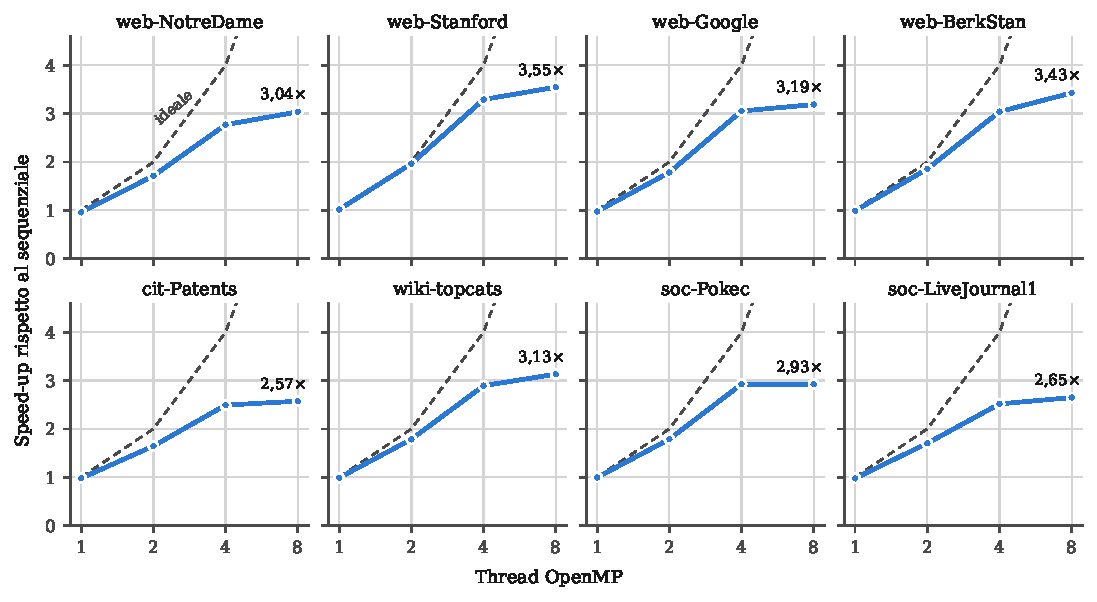
\includegraphics[width=\linewidth]{figure/scalabilita.pdf}
\caption{Scalabilità della versione OpenMP. Il riferimento per lo speed-up è
la build sequenziale vera, compilata senza \texttt{-fopenmp}. La linea
tratteggiata in (a) indica lo speed-up lineare ideale; in (b) l'efficienza
del 100\,\%. Su \texttt{web-Google} e \texttt{web-BerkStan} il passaggio da
4 a 8 thread \emph{peggiora} il tempo di esecuzione. Figura generata da
\texttt{tools/plot\_results.py} a partire da \texttt{results/bench.csv}.}
\label{fig:scalabilita}
\end{figure}

La Figura~\ref{fig:scalabilita} rende visibile il fenomeno descritto sopra:
le tre curve si allontanano dall'andamento lineare già a 2 thread e si
appiattiscono fra 4 e 8, con una vera e propria inversione su due grafi su
tre. L'efficienza scende dal 90\,\% circa a 2 thread al 70\,\% a 4, fino a
circa il 30\,\% a 8: i thread aggiuntivi non trovano banda di memoria
disponibile.

\paragraph{Osservazione principale: il calcolo è memory-bound.}
Su due grafi su tre l'esecuzione con 8 thread è \emph{più lenta} di quella
con 4. Il processore possiede 4 core fisici presentati come 8 thread
logici; i due thread che condividono un core condividono anche la via di
accesso alla memoria. Poiché il ciclo interno passa la maggior parte del
tempo in attesa di letture sparse su \texttt{contrib}, i thread aggiuntivi
producono contesa anziché capacità di calcolo.

L'efficienza parallela su 4 core è del 60--72\%. Questo risultato è il
dato più importante dell'analisi: identifica il collo di bottiglia nella
\emph{larghezza di banda della memoria}, non nella potenza di calcolo, e
costituisce la motivazione quantitativa per il passaggio alla GPU --- il cui
vantaggio non è tanto il maggior numero di core quanto la banda di memoria
sensibilmente superiore.

\paragraph{Nota sull'istanza più piccola.}
I tempi di \texttt{wiki-Vote} non sono riportati in
Tabella~\ref{tab:scaling}: con durate dell'ordine del millesimo di secondo
la dispersione fra ripetizioni della stessa configurazione raggiunge un
fattore $51\times$, il che significa che si misurerebbe l'avvio del team di
thread e non l'algoritmo. Il grafo resta nell'insieme di prova con il ruolo
di riferimento di correttezza (Sezione~\ref{sec:verifica}).

\subsection{Confronto fra le varianti \texttt{float} e \texttt{double}}
La variante in singola precisione è più rapida del $32\%$ su
\texttt{web-Google} ($0{,}347$~s contro $0{,}459$~s), a parità di numero di
iterazioni e con ranking identico. Il guadagno è coerente con il
dimezzamento dei byte trasferiti per ogni rank, ed è un'ulteriore conferma
indiretta della natura memory-bound del calcolo.

Il limite della singola precisione si manifesta sulla soglia di
convergenza: su \texttt{web-Google} l'errore $L_1$ non scende sotto
$\approx 5\cdot10^{-9}$, per cui una tolleranza di $10^{-9}$ non viene mai
raggiunta mentre la doppia precisione converge in 104 iterazioni. Alla
tolleranza utilizzata negli esperimenti ($10^{-6}$) entrambe convergono
nello stesso numero di iterazioni.

\subsection{Risultati della versione ibrida}
\daFare{Sezione da scrivere: tempi della versione CUDA e ibrida, confronto
con OpenMP, occupancy, effetto della granularità adattiva, effetto della
sovrapposizione fra trasferimenti e calcolo.}

% =====================================================================
\section{Valutazioni e osservazioni}
% =====================================================================

\subsection{Punti di forza}
\begin{itemize}
  \item \textbf{Assenza di sincronizzazione nel nucleo di calcolo.} La
    scelta del CSR trasposto elimina alla radice le scritture concorrenti,
    e si trasferisce invariata alla versione CUDA.
  \item \textbf{Riferimento sequenziale onesto.} Sequenziale e parallelo
    provengono dallo stesso sorgente, il che rende impossibile una
    divergenza fra le due versioni e non gonfia lo speed-up dichiarato.
  \item \textbf{Verifica indipendente e collaudata.} Tre implementazioni
    concordano, e lo strumento di verifica è stato validato con
    un'iniezione di guasto.
  \item \textbf{Riproducibilità.} L'intera campagna sperimentale è
    riproducibile con un solo comando.
\end{itemize}

\subsection{Punti deboli e limiti}
\begin{itemize}
  \item \textbf{Il convertitore non scala oltre le istanze usate.} Il
    convertitore Python mantiene l'intera edge list in memoria, con un costo
    di circa 100 byte per arco (6,66~GB misurati su
    \texttt{soc-LiveJournal1}). Un'istanza da un miliardo di archi
    richiederebbe un convertitore in C con ordinamento esterno.
  \item \textbf{Formato binario non standard.} Il formato \texttt{.csr} è
    specifico del progetto: è velocissimo da caricare, ma non ispezionabile
    con strumenti esterni. La scelta è stata fatta consapevolmente,
    privilegiando l'assenza di parsing nel percorso misurato.
  \item \textbf{Dimensione della porzione dinamica non ottimizzata.} Il
    valore 256 di \texttt{schedule(dynamic, 256)} non è stato oggetto di
    una ricerca sistematica.
\end{itemize}

\subsection{Possibili miglioramenti}
\begin{itemize}
  \item \textbf{Gestione out-of-core.} Era prevista in fase di proposta una
    logica di streaming per grafi eccedenti la memoria della GPU. Le misure
    hanno mostrato che non è necessaria per le istanze considerate: il
    grafo più grande occupa 356~MB contro i 4~GB disponibili, e servirebbe
    un'istanza dell'ordine del miliardo di archi per superare la soglia.
    Resta un possibile sviluppo futuro, subordinato però alla riscrittura
    del convertitore.
  \item \textbf{Granularità adattiva sulla GPU.} Le misure di
    Tabella~\ref{tab:bins} sono già disponibili ma non ancora sfruttate da
    alcun kernel.
  \item \textbf{Ricerca sui parametri di scheduling} (politica e dimensione
    del blocco) e confronto con \texttt{guided}.
\end{itemize}

\daFare{Aggiungere la valutazione personale complessiva una volta
completata la fase CUDA.}

% =====================================================================
\section{Guida all'uso e riproducibilità}
% =====================================================================

\subsection{Requisiti}
\texttt{gcc} con supporto OpenMP; CUDA Toolkit per la versione ibrida;
Python~3 con \texttt{numpy} per la conversione dei dataset,
più \texttt{networkx} e \texttt{scipy} per la sola verifica di correttezza.

\subsection{Compilazione}
\begin{lstlisting}[language=bash,numbers=none]
make
\end{lstlisting}
Produce quattro eseguibili in \texttt{build/}: \texttt{pagerank\_seq}
(senza OpenMP), \texttt{pagerank\_omp}, \texttt{pagerank\_omp\_float} e
\texttt{csr\_info}. Tutti derivano dagli stessi file sorgente.

\subsection{Preparazione dei dati}
\begin{lstlisting}[language=bash,numbers=none]
mkdir -p data/snap && cd data/snap
for g in wiki-Vote web-Google web-BerkStan soc-LiveJournal1; do
    curl -O https://snap.stanford.edu/data/$g.txt.gz && gunzip $g.txt.gz
done
cd ../..
python3 tools/snap_to_csr.py data/snap/web-Google.txt
\end{lstlisting}

\subsection{Esecuzione}
\begin{lstlisting}[language=bash,numbers=none]
./build/pagerank_omp data/snap/web-Google.csr -i data/snap/web-Google.ids
\end{lstlisting}
Opzioni: \texttt{-d} damping, \texttt{-t} tolleranza, \texttt{-n} iterazioni
massime, \texttt{-k} quanti nodi stampare, \texttt{-o} salva tutti i rank,
\texttt{-c} accoda una riga CSV con i dati dell'esecuzione. Il numero di
thread si imposta con \texttt{OMP\_NUM\_THREADS}.

\subsection{Verifica della correttezza}
\begin{lstlisting}[language=bash,numbers=none]
python3 tools/verify_pagerank.py data/snap/wiki-Vote.txt
\end{lstlisting}
Termina con stato diverso da zero in caso di discrepanza, e può quindi
essere usato come test di regressione.

\subsection{Riproduzione degli esperimenti}
\begin{lstlisting}[language=bash,numbers=none]
tools/run_benchmarks.sh
\end{lstlisting}
Esegue ogni grafo con le varianti sequenziale, OpenMP (1/2/4/8 thread) e
\texttt{float}, con tre ripetizioni, e scrive \texttt{results/bench.csv}
(una riga per esecuzione) e i vettori dei rank completi. Le impostazioni
sono sovrascrivibili da ambiente, ad esempio
\texttt{GRAPHS="wiki-Vote" REPS=1 tools/run\_benchmarks.sh}.

\subsection{Codice sorgente}
Il codice completo, con la cronologia di sviluppo, è disponibile all'indirizzo
\begin{center}
\url{https://github.com/EmanueleCecchia/pagerank-openmp-cuda}
\end{center}
Il repository contiene i sorgenti C, gli strumenti Python di conversione e
verifica, lo script della campagna sperimentale e il file
\texttt{results/bench.csv} con i dati grezzi di tutte le esecuzioni. I
dataset e i vettori dei rank non sono versionati per ragioni di dimensione:
i primi si riscaricano con i comandi della Sezione~5.3, i secondi si
rigenerano con \texttt{tools/run\_benchmarks.sh}.

% =====================================================================
\begin{thebibliography}{9}
\bibitem{page1999} L.~Page, S.~Brin, R.~Motwani, T.~Winograd,
  \emph{The PageRank Citation Ranking: Bringing Order to the Web},
  Stanford InfoLab, 1999.
\bibitem{visali2024} V.~Visali, R.~Manimegalai, S.~Noor Mahammad,
  A.~Sunitha Nandhini, \emph{Performance Analysis of Parallelized PageRank
  Algorithm using OpenMP, MPI and CUDA}, ICSSEECC, pp.~44--49, IEEE, 2024.
\bibitem{snap} J.~Leskovec, A.~Krevl, \emph{SNAP Datasets: Stanford Large
  Network Dataset Collection}, \url{https://snap.stanford.edu/data}, 2014.
\bibitem{kirk2016} D.~B.~Kirk, W.~W.~Hwu, \emph{Programming Massively
  Parallel Processors}, 3rd ed., Morgan Kaufmann, 2016.
\bibitem{cuda} NVIDIA, \emph{CUDA C++ Programming Guide}.
\end{thebibliography}

\end{document}
